\documentclass[a4paper,fleqn,usenatbib]{mnras}

\usepackage{newtxtext,newtxmath}
% Depending on your LaTeX fonts installation, you might get better results with one of these:
%\usepackage{mathptmx}
%\usepackage{txfonts}

\usepackage[T1]{fontenc}
\usepackage{ae,aecompl}

\usepackage{numprint}
\usepackage{booktabs}
\usepackage{float}

\usepackage{amsbsy}
\usepackage{graphicx}	% Including figure files
\usepackage{color}
\usepackage{amsmath}	% Advanced maths commands
\usepackage{amssymb}	% Extra maths symbols

\newcommand{\todo}[1]{\textcolor{red}{#1}}

%%%%%%%%%%%%%%%%%%%%%%%%%%%%%%%%%%%%%%%%%%%%%%%%%%

%%%%% AUTHORS - PLACE YOUR OWN COMMANDS HERE %%%%%

% Please keep new commands to a minimum, and use \newcommand not \def to avoid
% overwriting existing commands. Example:
%\newcommand{\pcm}{\,cm$^{-2}$}	% per cm-squared

%%%%%%%%%%%%%%%%%%%%%%%%%%%%%%%%%%%%%%%%%%%%%%%%%%


% Title of the paper, and the short title which is used in the headers.
% Keep the title short and informative.

\title[Discovery and origin of $r$-process stars]{On the discovery and origin of $r$-process stars in the Milky Way}

% The list of authors, and the short list which is used in the headers.
% If you need two or more lines of authors, add an extra line using \newauthor
\author[Matthew T. Miles et al.]{Matthew T. Miles,$^{1}$\thanks{E-mail: mtmil3@student.monash.edu}
	Andrew R. Casey,$^{1,2}$
	Brodie J. Norfolk,$^{1}$
	Alex J. Kemp,$^{1}$\newauthor
    Joss Bland-Hawthorn?,$^3$
    Anna Y. Q. Ho?,$^4$
    Alexander P. Ji?,$^5$
	John C. Lattanzio?,$^{1}$\newauthor
	Kevin C. Schlaufman?,$^{6}$
	\\
	% List of institutions
	$^{1}$School of Physics and Astronomy, Monash University, Clayton Campus, Victoria 3800, Australia\\
	$^{2}$Faculty of Information Technology, Monash University, Clayton Campus, Victoria 3800, Australia\\
    $^{3}$Sifa, University of Sydney\\
	$^{4}$Cahill Center for Astrophysics, California Institute of Technology, MC 249-17, 1200 E California Blvd, Pasadena, CA, 91125, USA\\
    $^{5}$Carnegie Observatories\\
    $^{6}$Department of Physics and Astronomy, Johns Hopkins University, 3400 N Charles St., Baltimore, MD 21218, USA
}

\date{Accepted XXX. Received YYY; in original form ZZZ}

\pubyear{2018}

\begin{document}
	\label{firstpage}
	\pagerange{\pageref{firstpage}--\pageref{lastpage}}
	\maketitle
	
	\begin{abstract}
		The production of heavy elements occurs through the slow and rapid neutron capture process. Numerous sites satisfy the conditions needed for the r-process but the relative frequency of these sites is unknown, largely due to the lack of a large number of stars with strong r-process signatures. Here we report the discovery of 47 r-process enhanced stars discovered in the second LAMOST data release (DR2), more than doubling the known number in the Galaxy. Taking expected rates of core-collapse supernovae and the average r-process material ejected per event, we find that core-collapse supernovae alone cannot explain the number of r-process stars discovered in this work within the lifetime of the universe. Current estimates of neutron-star merger rates imply that there should be about 13,000 r-process enhanced stars in the Milky Way, and about $79$ in LAMOST DR2. We find that neutron-star mergers are able to create all currently known r-process enhanced stars within about 10\,Gyr. To our knowledge, this is the first work that links the rates of neutron-star mergers to the number of r-process stars in the Milky Way. All 47 r-process enhanced stars have $[{\rm Fe/H}] > -2$, providing the first evidence against the hypothesis that r-process signatures are only found in poor metallicity environments.
	\end{abstract}
	
	\begin{keywords}
		nucleosynthesis -- r-process -- neutron-star mergers -- core-collapse supernovae
	\end{keywords}
	
	
	\section{Introduction}
	
	Heavy elements ($Z > 30$) are synthesised through the slow (s) and rapid (r) neutron capture processes \citep[e.g.,][]{Burbidge1957,Sneden2008}.
	Rapid neutron capture occurs when the neutron density is high enough such that the rate of neutron capture will occur faster than the rate at which an isotope undergoes a $\beta$-decay. Extremely high neutron densities ($>$$10^{24}\ \rm{free\ neutrons\ per\ cm}^{3}$) are necessary for the r-process to occur. Sites meeting this criteria include core-collapse supernovae (especially those that are magnetorotationally driven), neutron-star mergers. Core-collapse supernovae are believed to be relatively common throughout the history of the Milky Way, but they only produce small amounts of r-process material. Neutron-star mergers or magnetorotationally driven supernovae, however, occur much less frequently than ordinary core-collapse supernovae, but produce far more r-process material. Events such as these are theorised to account for the case of the highly r-process enhanced stars in the ultra-faint dwarf (UFD) galaxy Reticulum II \citep{Ji2016}.
	Magnetorotationally driven supernovae may not produce as much r-process material as neutron-star mergers (although still more than ordinary core-collapse supernovae), but are thought to occur more frequently than neutron-star mergers \citep[e.g.,][]{Li2011, LIGO2016}, and the predicted abundance patterns make them observationally indistinguishable from neutron-star mergers \citep{Ji2016}.
	
	Europium ($Z=63$) is almost entirely produced through the r-process. This makes it a very useful signature for identifying stars that show evidence of a significant contribution from r-process material. Using europium as a tracer, \cite{Ji2016} found that the level of r-process enrichment in  Reticulum II was too high to have occurred through a single core-collapse supernovae event.
	Historically, UFD galaxies have demonstrated some of the lowest abundance ratios of r-process elements with respect to Fe seen in the Milky Way or its satellite systems. However, the analysis of several of Reticulum II's stars show they are greatly enriched in r-process elements, 2-3 orders of magnitude higher than stars found in any other UFD galaxy \citep{Ji2016}. This degree of enrichment supports the theory that a single rare event must have occurred early on in the formation history of Reticulum II. This is supported by the observed heavy element yields, which are found to be some 1000 times higher than what is achievable on average from core-collapse supernovae ejecta. It is highly improbable that 1000 supernovae could have contributed to Reticulum II, suggesting that the r-process material must be produced by a rarer astrophysical event such as a binary neutron-star merger.
	
	While neutron-star mergers or magnetorotationally driven supernovae are likely to produce significant amounts of r-process material, it does not suggest that all r-process material stems from these sources either. Rather, the rarity of these events might imply that they are also responsible for the rare numbers of stars  observed to have significant enhancements in r-process material. One could ask if neutron-star mergers could be responsible for all r-process stars known in the Milky Way? On the other hand, if we assume very little gas mixing, could core-collapse supernovae create enough material to explain a single r-process enriched star? If neither of these prove to be true then we can confirm that there must be multiple sites to the r-process, providing a step forward in understanding the relative fraction of these mechanisms in the Milky Way.
	
	In order to answer these questions it is necessary to identify a large sample of r-process stars.
	However, r-process stars are very rare. For this reason we must look to massive data sets, such as the LAMOST sky survey. In this letter we report the discovery of 47 r-process enhanced stars identified from LAMOST, significantly building upon the previously known Milky Way sample of 26 \citep[e.g.,][]{masho2011,Honda2004,Hayek2009,Sneden2003,Ivans2006,Hill2002,Christlieb2004,Wako2010,placo2017,Sakari2018}.
	In Section 2 we outline the methods used to identify r-process enhanced candidates, and our analysis methods. In Section 3 we discuss what our results imply about the sites of the r-process. We provide concluding remarks in Section 4.
	
	
	\begin{figure*}
		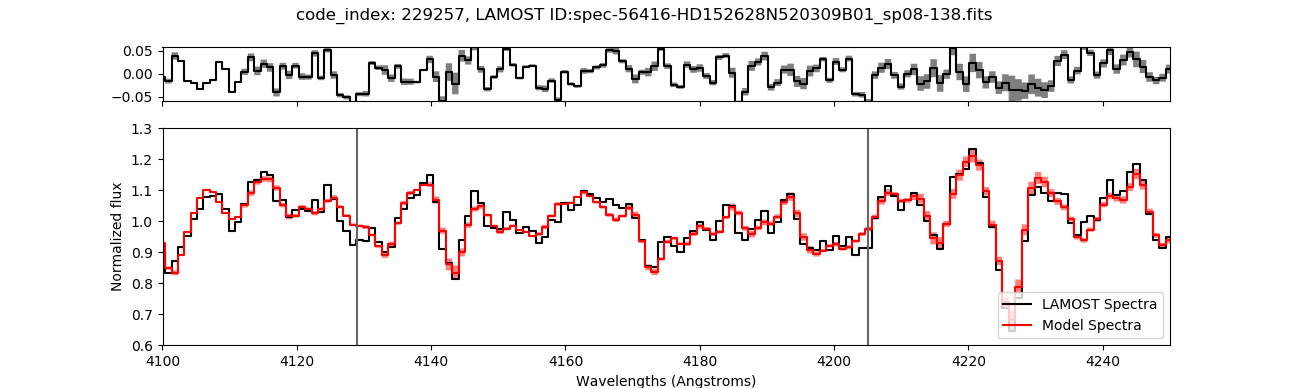
\includegraphics[width=\textwidth]{229257}
		\caption{The spectral region around two Europium absorption lines at 4129 and 4205 Angstroms. This particular star's spectra (black) shows clear absorption at these wavelengths, as compared to the data-driven model (red).}
		\label{fig:starindex_229257}
	\end{figure*}
	
	\begin{figure}
		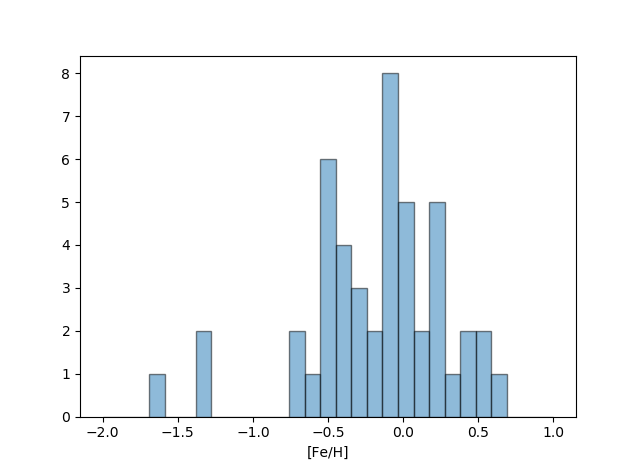
\includegraphics[width=\columnwidth]{metalhistpython}
		\caption{The metallicities of the 47 candidate stars.}
		\label{fig:metallicity}
	\end{figure}
	
	\section{Methods}
	
	\subsection{Observations and Candidate Selection}
	
	The LAMOST survey is a low resolution optical spectroscopic survey ($R\approx1800$; 3650-9000\,\AA). The second data release from LAMOST \citep{lamost} contains about 2.2 million stellar spectra in the northern sky. Of these 2.2 million, 454,180 were identified as giant stars through a data-driven analysis known as \textit{The Cannon} \citep{AnnaHo2017}. An overlap sample of 9,952 giant stars common to LAMOST and the higher-resolution ($R\approx22500$) APOGEE survey \citep{apogee} were used as a training set.
	The stellar labels included in \textit{The Cannon} model are stellar effective temperature $T_{\rm{eff}}$, surface gravity $\log{g}$, overall metallicity $\rm{[Fe/H]}$, average relative abundance of elements produced via $\alpha$-particle capture $\rm{[\alpha/Fe]}$, and K-band extinction $\rm{A_{k}}$. For reference, typical uncertainties for these labels are about $70\,\rm{K}$ for $T_{\rm{eff}}$, $0.1$ in $\log{g}$, 0.1\, in $\rm{[Fe/H]}$, and 0.04\, in $\rm{[\alpha/Fe]}$.
	
	We identified candidate r-process enhanced stars by searching for deviations between the pseudo-continuum-normalised flux and the best-fitting data-driven model spectrum. Specifically, we looked for deviations at the 4129\,\AA\ and 4205\,\AA\ europium absorption lines. At each transition we fitted a Gaussian profile to the flux residuals for all 454,180 giant stars. We recorded the amplitude, wavelength, and width of each profile, as well as the corresponding uncertainties on these quantities. 
	Candidate r-process stars were identified as stars that met the following criteria:
	
	\begin{itemize}
		\item The amplitude $\rm{A}$ of the fitted gaussian profile must be ${A<-0.05}$;
		\item The signal to noise (S/N) must be greater than 30;
		\item The deviation from the required wavelength in question must be less than 2\,\AA;
		\item The reduced $\chi_r^{2}$ value must be less than 3, $\chi_r^{2}<3$.
		\item All of these conditions must be met for both 4129\,\AA\ and 4205\,\AA\ for us to consider them sufficiently Eu enhanced.
	\end{itemize}   
	
	These filters produced an initial sample of 62 candidates from the total sample of 454,180. An example candidate is shown in Figure \ref{fig:starindex_229257}. We visually scrutinised each candidate to remove false positives, typically due to data reduction artefacts. After this process we were left with 47 likely r-process enhanced candidates, 22 of which stand out as very strong candidates. In addition to this we searched these stars for enhancements of a similar degree in the s-process created elements Strontium and Barium and found none. 
	
	\section{Identifying the r-process}
	
	\subsection{Selection effects}
	The LAMOST giants we analyse belong to a broad range of metallicity ($-1.6 < \rm{[Fe/H]} < 0.6$), and don't cluster in any part of the sky, suggesting they do not belong to a single stellar system. The lowest metallicity among the 454,180 giant stars in our sample is $[{\rm Fe/H}] \approx -2.1$. The previous sample of known r-process stars, before this work, exclusively consists of very metal-poor stars with $[{\rm Fe/H}] < -1.5$ \citep{Barklem2005}. This fact is not to be confused with saying that most r-process stars found should be metal-poor stars, rather that at extremely low metallicities of $[{\rm Fe/H}] \lesssim -2.6$ \citep{Simmerer2004} there is a negligible contribution from the s-process
	and all neutron-capture elements must be formed from the r-process. In other words, the primary reason why all r-process enhanced stars have $[{\rm Fe/H}] < -2$ is simply because searches for r-process stars have primarily focussed in the low metallicity regime.
	
	
	%Over half the current known r-process stars are members of the ultra faint dwarf galaxy, Reticulum II. %However, europium we know to be totally made from the r-process, therefore even at metallicities where the s-process contributes, Europium is a valuable indicator of r-process synthesis.
	
	\subsection{Multiple r-process sites?}
	While it is possible that all known r-process enhanced stars could be made by neutron-star mergers (we show this in Section \ref{rates}), we also observe stellar populations in the galaxy which show relatively weak enrichment from r-process elements ($[{\rm Eu/Fe}] < 0.7$). These enhancements imply either that there is more than one active r-process site, or that there is a very heterogeneous level of gas mixing, such that neutron-star mergers are able to enhance stars with [Eu/Fe] abundances that cover  many orders of magnitude.
	
	\subsection{Core-collapse supernovae}
	Core-collapse supernova are one of the sites initially proposed to have a high enough neutron density to create elements synthesised by the r-process \citep{Burbidge1957}. Currently, the exact  mechanism that creates material with a high enough neutron density to synthesise r-process material is unknown.
%	As of yet our knowledge is incomplete on the exact mechanism that allows material with a high enough neutron density to escape the supernovae event.
	One possible mechanism is the action of high-entropy neutrino winds being released from a proto-neutron-star during core-collapse. In this stage of the collapse, this neutrino wind is driving mass loss and could be instrumental in the expulsion of the r-process material in supernovae conditions. However, how much enhanced material is released from the event depends heavily on the amount of material that is allowed to fall back onto the remnant at the arrival of the reverse shock, and so often the supernovae may not release a considerable amount of material \citep{Woosley1992, Burrows1995}. 
	
	Regardless of the exact mechanism, core-collapse supernovae seem to release $M_{\rm{Eu}}\approx10^{-7.5} M_{\odot}$ per event \citep{Argast2004}. While this may not be a particularly significant mass of europium, core-collapse supernovae occur reasonably frequently \citep[44,700$\,\ \rm{Gpc}^{-3} \rm{yr^{-1}}$;][]{Li2011}, and so with little mixing core-collapse supernovae are a candidate as the progenitor for some r-process enhancements under the conditions listed, but it can not be the sole source.
	
	\subsection{Neutron-star mergers}
	\label{NSmerg}
	Neutron-star mergers are another possible site of r-process element nucleosynthesis \citep{Kasen2017,Hotok2013,Drout2017}. They satisfy the conditions necessary to create a high neutron density by means of interacting tidal forces between the stars, neutron dense material is accreted off the stars, allowing r-process element synthesis to occur. This specific process produces considerably more enriched material than core-collapse supernovae ($M_{\rm{Eu}}\approx10^{-4.5} M_{\odot}$) \citep{Goriely2011}, consistent with observed ejecta \citep{Kasliwal2017}. However, the direct interaction and merger of a binary neutron-star pair occurs very infrequently, with currently only one direct observation, and with a most plausible frequency estimate of 1,000$\,\rm{Gpc^{-3}yr^{-1}}$ \citep{LIGO2016,Abadie2010} well within the the outer estimates of $320 and 4780\ \rm{Gpc^{-3}yr^{-1}}$. The significant amount of material that these mergers release can compensate for their low frequency and so it could be that they are responsible for most if not all r-process enhancements observed.

	The recent discovery of the UFD Reticulum II \citep{Ji2016} is evidence against the case of a single r-process site. Of nine stars observed in Reticulum II, 7 of them were shown to be highly enriched in r-process elements ($\rm{[Eu/Fe]\approx1.7}$) which suggests a single prolific event having occurred in close proximity to the galaxy early in it's formation, such as a neutron-star merger. However, two of the stars observed were only weakly enhanced in r-process elements which suggests that there must have been a second, less efficient, form of r-process enhancement present.
	
	\subsection{The rates of r-process events and what they imply}
	\label{rates}
	From the recent advanced LIGO data \citep{LIGO2016}, we are able to find an estimate for a plausible frequency at which neutron-star mergers occur, as mentioned in Section \ref{NSmerg}. Reliable estimates of core-collapse supernovae are also available \citep{Li2011}. From these two rates we can estimate the amount of r-process enhanced giants that should be present in the Milky Way, either enhanced solely by purely neutron-star mergers, or purely by core-collapse supernovae. As well as an estimate of how many r-process enhanced stars, giants or dwarfs, that are expected to be present in the Milky Way. We assume instant recycling, and that no r-process matter pollutes stars by any other means than these two mechanisms. In these calculations a star is deemed to be 'enhanced' where $[{\rm Eu/Fe}] \geq 0.7$.
	
	Taking the mass of europium ejected from a neutron-star merger as $M_{\rm Eu}\approx10^{-4.5}\,M_{\odot}$, we can calculate a density of Europium $\rho_{\rm Eu}$,
\begin{equation}
	\centering
	\rho_{\rm Eu} = M_\textrm{Eu}\frac{dN}{dt}(13.87\times10^9\,{\rm yr})
\end{equation}

\noindent{}where ${dN}/{dt}$ is the estimated rate of neutron-star mergers (1,000$\,{\rm Gpc}^{-3}{\rm yr}^{-1}$). From this calculation we expect there to be present $\approx1.23 \times 10^{25}$ kilograms of Europium within a 15 kpc radius sphere from the centre of the Milky Way.
	
	The total known mass of Europium exhibited in these 47 stars was then calculated:
	\begin{equation}
	M_{\rm{Eu}} = 47*A_{\textrm{Eu}}*N_{\textrm{Eu}}
	\end{equation}
	Where:
	\begin{equation}
	Eu_{\rm{Atomic\ mass}} = 2.52342^{-25}
	\end{equation}
	\begin{equation}
	N_{\rm{Eu\ atoms}} = 10^{[Eu/H]-12} \times N_{\rm{Hydrogen\ atoms}}
	\end{equation}
	The number of Hydrogen atoms was approximated from the Hydrogen atomic mass, and the assumption was made that a giant star will be composed of $\approx$75\% Hydrogen and each star possesses an average mass of $\approx 0.8\ M_{\odot}$. [Eu/H] was found under the assumption the star would exhibit a [Eu/Fe] = 0.7, and using the [Fe/H] given in Table 1. These assumption mean that a Europium mass of $9.3 \times 10^{20}$ kilograms is required to be present in the star for it to be deemed 'enhanced'.
	
    It was found that in the Milky Way there should be present 13,060 r-process stars enhanced solely from neutron-star mergers. Taking into account that this should be considered a upper-bound estimate this is still a startlingly large difference from the known 73 r-process stars in the Milky Way.
    
    In preparing these calculations we assumed a constant star formation rate of 2 M$_\odot {\rm yr}^{-1}$ in the disk of the Milky Way, with a typical IMF and giant star birth rate of approximately 0.3 stars per year. Therefore if we assume a steady-state system, the number of red giant stars in the Milky Way comes to approximately $7.53\times10^7$. This allows us to find the fraction of the Milky Ways giants that our sample of r-process stars represents. Multiplying this fraction by the 13,060 stars that should be present in the Milky Way, we expect to be present 79 enhanced stars in LAMOST DR2, a number consistent with the 73 we now know of.
    
    %Scaling down from the 250 billion stars in the Milky Way to our sample size of $\approx450000$ giants, the amount of enhanced stars we expect to find comes to less than one (0.0178). If we are to extend our sample from the 450000 giants, and instead use the entire LAMOST data release 2 (a survey of $\approx2.2$ million stars), we predict that we should still have found less than a single star (0.087) enhanced in r-process elements. While again this should be considered a lower bound, it is nonetheless a startling difference from the 47 that were found.
    
    We can do a similar calculation with our rate of core-collapse supernovae. Taking the same assumptions with minimal mixing, as well as both the ejecta ($M_{Eu}\approx10^{-7.5} M_{\odot}$) and rate ($44700\ \rm{Gpc}^{-3} \rm{yr^{-1}}$) previously discussed, we find that in the Milky Way there should be present 584 r-process enhanced stars made solely from core-collapse supernovae. Applying the same method as utilised in the neutron-star merger calculations, we expect there to be present only 4 r-process enhanced stars in LAMOST DR2 enhanced entirely by core-collapse supernovae.
    
    %Were we to scale this down to our sample size of $\approx450000$ giants we arrive at a figure of $8.0\times10^{-4}$ stars that should have been observed. Scaling again to the full LAMOST sample we would then expect to find $3.9\times10^{-3}$ enhanced stars. 
    
    From these estimates we find an approximation for whether or not either neutron-star mergers or core-collapse supernovae by themselves are sufficient to enrich our entire r-process enhanced catalogue. 
    
    Following from the assumptions listed and calculations above, neutron-star mergers could create enough r-process material to enrich above the point of [Eu/Fe] > 0.7 for the 47 known r-process enhanced stars within the LAMOST sample within $10.9\times10^{9}$ years, very close to the age of the universe. From our rates of core-collapse supernovae however, we find that the earliest time-scale at which they can create this level of r-process material is $2.4\times10^{11}$ years, orders of magnitude longer than the age of the universe. This illustrates, with our current knowledge of core-collapse supernovae frequency, and the amount of r-process material they eject, that core-collapse supernovae cannot be the sole source of r-process enrichment in the Milky Way.
    
    This is reinforced by the r-process enhanced stars found in the LAMOST sample. Our 47 stars represent almost 10\% of all r-process enhanced stars present in the Milky Way if core-collapse supernovae is considered to be the singular source of r-process enhanced stars. However, the LAMOST data release 2 only surveyed a small fraction of the Milky Way. It is highly unlikely that close to 10\% of the entire r-process enhanced population of the Milky Way exists within our stellar sample. It is then concluded that core-collapse supernovae can not be the only source of r-process material. 
    
    In an effort to confirm these numbers, we approached the calculation from a different direction. Were we to take our sample of 47 giants found in the LAMOST data, and increase it to the full estimated amount of giants in the galaxy, then we would expect to find about 7,849 r-process enhanced giant stars, very close to the 13,060 stars from the previous calculation.
	
	\section{Conclusions}
	We present the largest sample of r-process element enhanced stars to date. Our sample is found to cover a wide range of metallicities, contrary to previous discoveries that focussed on metal-poor r-process enhanced stars. These 47 stars represent the first r-process enhanced stars found at [Fe/H] $>-2$. The sample is not grouped in effective temperatures, surface gravity, or radial velocity, and are not clustered in any  particular location on the sky. We present the first estimate, to our knowledge, that neutron-star mergers could synthesise all r-process material in the known r-process enhanced stars within the age of the universe. We also provide evidence to confidently conclude core-collapse supernovae can not possibly be the only progenitors of r-process material in the Milky Way Galaxy.
	
	We recommend follow-up high resolution spectra be obtained for each of the 47 stars to ascertain how enhanced they are. To find the origin of these stars and to show whether or not they may come from a similar progenitor site it is necessary to find orbits for them.
	
	
	% The best way to enter references is to use BibTeX:
	
	\bibliographystyle{mnras}
	%\bibliography{paper} % if your bibtex file is called example.bib
	\begin{thebibliography}{99}
		\bibitem[\protect\citeauthoryear{Abadie et al.}{2010}]{Abadie2010}
		Abadie J. et al. 2010, Classical and Quantum Gravity, 27, 17
		\bibitem[\protect\citeauthoryear{Abbott et al.}{2016}]{LIGO2016}
		Abbot B.P. et al. 2016, Living Reviews in Relativity, 19, 1
		\bibitem[\protect\citeauthoryear{Argast et al.}{2004}]{Argast2004}
		Argast D., Samland M., Thielmann F-K. \& Qian Y-Z. 2004, Astronomy and Astrophysics, 416
		\bibitem[\protect\citeauthoryear{Barklem et al.}{2005}]{Barklem2005}
		Barklem, P.S., Christlieb, N., Beers, T.C., Hill, V., Besel, M.S., Holmberg, J., Marsteller, B., Rossi, S., Zickgraf, F.-J. \& Reimers, D. 2005, A\&A, 439, 1
		\bibitem[\protect\citeauthoryear{Burbidge et al.}{1957}]{Burbidge1957}
		Burbidge E. M., Burbidge G. R., Fowler W. A., \& Hoyle F. 1957, Review of Modern Physics, 29, 4
		\bibitem[\protect\citeauthoryear{Burrows et al.}{1995}]{Burrows1995}
		Burrows, A., Hayes, J., \& Fryxell, Bruce A. 1992, ApJ, 450, 830
		\bibitem[\protect\citeauthoryear{Cui et al.}{2012}]{lamost}
		Cui, X.-Q. et al., Research in Astronomy and Astrophysics, 12, 9
		\bibitem[\protect\citeauthoryear{Drout et al.}{2017}]{Drout2017}
		Drout, M. R. et al. 2017, Science
		\bibitem[\protect\citeauthoryear{Christlieb et al.}{2004}]{Christlieb2004}
		Christlieb N. et al. 2004, Astronomy \& Astrophysics, 428, 1
		\bibitem[\protect\citeauthoryear{Goriely et al.}{2011}]{Goriely2011}
		Goriely S., Bauswein A. \& Janka H-T. 2011, , 738, L32
		\bibitem[\protect\citeauthoryear{Hayek et al.}{2009}]{Hayek2009}
		Hayek W., Wiesendahl U., Christlieb N., Eriksson K., Barklem P. S., Hill V., Beers T. C., Farouqi K., Pfeiffer B.,\& Kratz K.-L. 2009, Astronomy and Astrophysics, 504, 1
		\bibitem[\protect\citeauthoryear{Hill et al.}{2002}]{Hill2002}
		Hill V. et al. Astronomy \& Astrophysics, 387, 1
		\bibitem[\protect\citeauthoryear{Ho et al.}{2017}]{AnnaHo2017}
		Ho A. Y. Q., Ness M. K., Hogg D. W., Rix H-W., Liu C., Yang F., Zhang Y., Hou Y.,\& Wang Y. 2017, ApJ, 836, 1
		\bibitem[\protect\citeauthoryear{Honda et al.}{2004}]{Honda2004}
		Honda S., Aoki W., Kajino T., Ando H., Beers T. C., Izumiura H., Sadakane K. \& Takada-Hidai M. 2004, ApJ, 607, 1
		\bibitem[\protect\citeauthoryear{Hotokezaka et al.}{2013}]{Hotok2013}
		Hotokezaka K., Kiuchi K., Kyutoku K., Okawa H., Skiguchi Y., Shibata M., \& Taniguchi K. 2013, APS
		\bibitem[\protect\citeauthoryear{Ivans et al.}{2006}]{Ivans2006}
		Ivans I. I.,Simmerer J., Sneden C., Lawler J. E., Cowan J. J., Gallino R., \& Bisterzo S. 2006, ApJ, 645, 1
		\bibitem[\protect\citeauthoryear{Ji et al.}{2016}]{Ji2016}
		Ji A. P., Frebel A., Chiti A., \& Simon J. D. 2016, Nature, 531
		\bibitem[\protect\citeauthoryear{Kasen et al.}{2017}]{Kasen2017}
		Kasen D., Metzger B., Barnes J., Quataert E., \& Ramirez-Ruiz E. 2017, Nature, 551, 7678
		\bibitem[\protect\citeauthoryear{Kasliwal et al.}{2017}]{Kasliwal2017}
		Kasliwal M. M., et al. 2017, Science,
		\bibitem[\protect\citeauthoryear{Lai et al.}{2008}]{Lai2008}
		Lai D. K., Bolte M., Johnson J. A., Lucatello S., Heger A., \& Woosley S. E. 2008, ApJ, 681,
		\bibitem[\protect\citeauthoryear{Li et al.}{2011}]{Li2011}
		Li W., Chornock R., Leaman J., Filippenko A. V., Poznanski D., Wang X., Ganshalingam M., \& Mannucci F. 2011, Royal Astronomical Society, 412, 1473
		\bibitem[\protect\citeauthoryear{Majewski et al.}{2017}]{apogee}
		Majewski S.R., et al., The Astronomical Journal, 154, 3
		\bibitem[\protect\citeauthoryear{Mashonkina et al.}{2010}]{masho2011}
		Mashonkina L., Christlieb N., Barklem P.S., Hill V., Beers T.C., \& Velichko A., Astronomy and Astrophysics, 516, 46
		\bibitem[\protect\citeauthoryear{Placco et al.}{2017}]{placo2017}
		Placco V.M., Holmbeck E. M., Frebel A., Beers T. C., Surman R. A., Ji A. P., Ezzeddine R., Points S. D., Kaleida C. C. Hansen T. T., Sakari C. M, \& Casey A. R., ApJ, 844, 1
		\bibitem[\protect\citeauthoryear{Simmerer et al.}{2004}]{Simmerer2004} Simmerer, J., Sneden, C., Cowan, J.~J., et al.\ 2004, \apj, 617, 1091 
		\bibitem[\protect\citeauthoryear{Sakari et al.}{2018}]{Sakari2018} Sakari C.M., et al. 2004, \apj, 854, 2
		\bibitem[\protect\citeauthoryear{Sneden et al.}{2008}]{Sneden2008}
		Sneden C., Cowan J.J., \& Gallino R. 2008, Annual review of Astronomy \& Astrophysics, 46, 1
		\bibitem[\protect\citeauthoryear{Sneden  et al.}{2003}]{Sneden2003}
		Sneden C. et al. 2003, ApJ, 591, 2
		\bibitem[\protect\citeauthoryear{Wako  et al.}{2010}]{Wako2010}
		Wako A., Beers T. C., Honda S. \& Carollo D. 2010, ApJ, 723, 1
		\bibitem[\protect\citeauthoryear{Woosley  et al.}{1992}]{Woosley1992}
		Woosley S.E, \& Hoffman R.D. 1992, ApJ, 395, 1
	\end{thebibliography}
	
	% Please add the following required packages to your document preamble:
	% \usepackage{booktabs}
	% Please add the following required packages to your document preamble:
	% \usepackage{booktabs}
	\begin{table*}
		\centering
		\label{Data for the 47}
		\begin{tabular}{@{}cccccccccccc@{}}
			\toprule
			\textbf{2MASS ID}   & \textbf{RA} & \textbf{DEC} & \textbf{S/N}        	& \textbf{$\boldsymbol{V_{\rm{r}}}$}   & \textbf{$\boldsymbol{T_{\rm{eff}}}$} & \textbf{Log(g)}	& \textbf{$\boldsymbol{[\rm{Fe/H}]}$} & \textbf{$\boldsymbol{[\alpha/\rm{H}]}$} & \textbf{$\boldsymbol{\chi_{\rm{r}}^{2}}$} & \textbf{{[}Eu/Fe{]}} & \textbf{Error} \\
			-               	& {[}H:M:S{]}   & {[}H:M:S{]}	& {[}$\rm{pixel}^{-1}${]} & {[}$\rm{km\ s}^{-1}${]} & {[}K{]}             	& {[}$\rm{cm\ s}^{-2}${]} & {[}dex{]}          	& {[}dex{]}              	& -                        	& {[}dex{]}        	& {[}dex{]}  	\\ \midrule
			J130303.65+260837.0 & 13:03:03.65 & +26:08:37.0  & 36.48               	& -37.77              	& 4851.24             	& 2.98           	& -0.54              	& 0.19                   	& 0.42                     	& 1.39             	& 0.31       	\\
			J062733.76+280814.1 & 06:27:33.77 & +28:08:14.2  & 39.08               	& 38.67               	& 4502.58             	& 1.92           	& -0.15              	& 0.00                   	& 0.35                     	& 1.43             	& 0.35       	\\
			J070035.19+103443.5 & 07:00:35.19 & +10:34:43.5  & 41.77               	& 17.69               	& 4752.08             	& 2.44           	& -0.43              	& 0.06                   	& 0.33                     	& 1.09             	& 0.63       	\\
			J070107.18+125948.2 & 07:01:07.19 & +12:59:48.2  & 33.72               	& 46.17               	& 4452.61             	& 2.51           	& 0.47               	& 0.02                   	& 0.36                     	& 1.30             	& 0.31       	\\
			J063400.95+420904.3 & 06:34:00.96 & +42:09:04.4  & 34.09               	& 9.89                	& 4315.56             	& 1.62           	& -0.50              	& 0.10                   	& 0.43                     	& 1.19             	& 3.10       	\\
			J220118.66+033558.6 & 22:01:18.66 & +03:35:58.6  & 35.11               	& -108.23             	& 4790.06             	& 2.51           	& -1.36              	& 0.33                   	& 0.37                     	& 1.44             	& 0.26       	\\
			J221220.27+032735.4 & 22:12:20.27 & +03:27:35.5  & 35.16               	& -12.89              	& 4867.34             	& 3.12           	& 0.11               	& 0.14                   	& 0.35                     	& 1.52             	& 0.20       	\\
			J060021.29+384840.6 & 06:00:21.29 & +38:48:40.6  & 30.03               	& 32.68               	& 4305.08             	& 2.10           	& 0.15               	& -0.01                  	& 0.54                     	& 1.49             	& 0.35       	\\
			J081632.10-053703.4 & 08:16:32.11 & -05:37:03.4  & 59.16               	& 44.67               	& 4541.14             	& 2.45           	& 0.57               	& 0.03                   	& 0.75                     	& 1.34             	& 0.26       	\\
			J064641.14+235318.2 & 06:46:41.14 & +23:53:18.3  & 36.77               	& 25.78               	& 4325.56             	& 1.78           	& -0.10              	& 0.02                   	& 0.42                     	& 1.41             	& 0.27       	\\
			J025225.88+324308.1 & 02:52:25.88 & +32:43:08.2  & 34.79               	& 24.88               	& 4797.58             	& 2.52           	& -0.23              	& 0.05                   	& 0.24                     	& 1.31             	& 0.29       	\\
			J061822.02+015126.7 & 06:18:22.02 & +01:51:26.8  & 36.75               	& 45.27               	& 4617.95             	& 2.43           	& -0.12              	& 0.04                   	& 0.34                     	& 1.42             	& 0.30       	\\
			J083049.21+304144.3 & 08:30:49.21 & +30:41:44.3  & 39.5                	& -125.31             	& 4859.92             	& 2.28           	& -1.63              	& 0.33                   	& 0.41                     	& 1.52             	& 0.20       	\\
			J035949.12+302104.4 & 03:59:49.13 & +30:21:04.4  & 30.42               	& 26.98               	& 4164.41             	& 1.79           	& -0.12              	& 0.00                   	& 0.36                     	& 1.47             	& 0.32       	\\
			J074852.24+075016.5 & 07:48:52.25 & +07:50:16.6  & 33.47               	& 36.87               	& 4405.84             	& 1.94           	& -0.48              	& 0.07                   	& 0.30                     	& 1.44             	& 0.30       	\\
			J163116.81+002349.5 & 16:31:16.81 & +00:23:49.5  & 32.63               	& -35.98              	& 4628.92             	& 2.53           	& 0.01               	& 0.18                   	& 0.29                     	& 1.44             	& 0.32       	\\
			J073532.54+215850.0 & 07:35:32.55 & +21:58:50.0  & 35.61               	& 35.98               	& 4859.66             	& 3.27           	& 0.19               	& 0.06                   	& 0.44                     	& 1.19             	& 0.79       	\\
			J164023.01+164552.5 & 16:40:23.02 & +16:45:52.6  & 44.59               	& -34.18              	& 4964.91             	& 2.96           	& 0.36               	& 0.07                   	& 0.35                     	& 1.27             	& 0.32       	\\
			J153333.12+510621.8 & 15:33:33.13 & +51:06:21.9  & 49.45               	& -17.99              	& 4861.78             	& 2.51           	& -0.49              	& 0.22                   	& 0.46                     	& 1.31             	& 0.28       	\\
			J175737.71+521523.1 & 17:57:37.71 & +52:15:23.2  & 38.52               	& -40.47              	& 4861.38             	& 3.36           	& -0.34              	& 0.10                   	& 0.55                     	& 1.51             	& 0.24       	\\
			J184125.86+432807.8 & 18:41:25.86 & +43:28:07.9  & 46.94               	& -93.84              	& 4703.92             	& 2.61           	& -0.26              	& 0.27                   	& 0.33                     	& 1.20             	& 0.34       	\\
			J195234.41+470859.4 & 19:52:34.41 & +47:08:59.5  & 68.57               	& -24.28              	& 4596.44             	& 2.54           	& 0.55               	& 0.07                   	& 0.82                     	& 0.95             	& 0.48       	\\
			J215146.68+304016.0 & 21:51:46.68 & +30:40:16.0  & 73.25               	& -28.78              	& 4566.21             	& 2.48           	& 0.64               	& 0.04                   	& 0.71                     	& 0.88             	& 0.45       	\\
			J075116.55+220137.8 & 07:51:16.56 & +22:01:37.9  & 32.87               	& 90.24               	& 4810.60             	& 2.70           	& -0.33              	& 0.02                   	& 0.30                     	& 1.35             	& 0.31       	\\
			J003929.43+430039.5 & 00:39:29.43 & +43:00:39.6  & 33.14               	& -104.33             	& 4190.26             	& 1.87           	& -0.01              	& 0.07                   	& 0.41                     	& 1.35             	& 0.33       	\\
			J040122.07+461504.5 & 04:01:22.08 & +46:15:04.5  & 35.43               	& -95.03              	& 4305.88             	& 1.75           	& 0.02               	& 0.10                   	& 0.57                     	& 1.37             	& 0.35       	\\
			J040815.45+464920.1 & 04:08:15.46 & +46:49:20.1  & 33.05               	& 16.19               	& 4855.16             	& 2.65           	& -0.11              	& 0.00                   	& 0.30                     	& 1.48             	& 0.30       	\\
			J071206.83+213038.0 & 07:12:06.84 & +21:30:38.1  & 32.66               	& 29.08               	& 4432.03             	& 1.75           	& -0.38              	& 0.11                   	& 0.40                     	& 1.47             	& 0.28       	\\
			J222820.22+340750.3 & 22:28:20.22 & +34:07:50.3  & 34.52               	& -45.27              	& 4419.96             	& 2.06           	& -0.07              	& 0.11                   	& 0.49                     	& 1.37             	& 0.31       	\\
			J222310.49+344357.4 & 22:23:10.50 & +34:43:57.5  & 54.06               	& -20.09              	& 4232.66             	& 1.87           	& -0.01              	& 0.03                   	& 0.86                     	& 1.22             	& 0.31       	\\
			J222101.61+365923.6 & 22:21:01.62 & +36:59:23.7  & 30.81               	& -27.88              	& 4360.28             	& 2.23           	& 0.20               	& 0.04                   	& 0.45                     	& 1.47             	& 0.29       	\\
			J052327.44+571126.8 & 05:23:27.45 & +57:11:26.8  & 33.54               	& -24.88              	& 4806.24             	& 3.08           	& 0.24               	& 0.07                   	& 0.45                     	& 1.43             	& 0.25       	\\
			J235212.27+492548.4 & 23:52:12.27 & +49:25:48.4  & 39.93               	& -95.03              	& 5047.36             	& 3.30           	& -0.43              	& 0.22                   	& 0.29                     	& 1.28             	& 0.26       	\\
			J074102.63+130520.3 & 07:41:02.64 & +13:05:20.4  & 40.83               	& 49.17               	& 5000.84             	& 3.00           	& -0.38              	& -0.02                  	& 0.30                     	& 1.35             	& 0.27       	\\
			J061559.10+470344.9 & 06:15:59.11 & +47:03:44.9  & 36.84               	& -18.29              	& 4811.98             	& 2.82           	& -0.59              	& 0.07                   	& 0.44                     	& 1.00             	& 1.33       	\\
			J054704.12+600827.1 & 05:47:04.13 & +60:08:27.1  & 33.19               	& -23.33              	& 4770.80             	& 2.64           	& -0.10              	& 0.06                   	& 0.40                     	& 1.46             	& 0.26       	\\
			J055548.33+611537.1 & 05:55:48.33 & +61:15:37.1  & 33.6                	& -40.88              	& 4850.39             	& 2.57           	& -0.46              	& 0.13                   	& 0.22                     	& 1.42             	& 0.26       	\\
			J042723.73+271546.8 & 04:27:23.73 & +27:15:46.9  & 45.73               	& -40.17              	& 4211.91             	& 1.72           	& -0.04              	& 0.05                   	& 0.79                     	& 1.33             	& 0.34       	\\
			J035702.05+281335.2 & 03:57:02.06 & +28:13:35.3  & 31.82               	& -44.67              	& 4712.89             	& 2.44           	& 0.01               	& 0.16                   	& 0.46                     	& 1.28             	& 0.38       	\\
			J031030.13+531759.9 & 03:10:30.13 & +53:17:59.9  & 35.34               	& -16.79              	& 4699.75             	& 2.34           	& 0.21               	& 0.00                   	& 0.89                     	& 1.51             	& 0.21       	\\
			J091256.32+353008.3 & 09:12:56.32 & +35:30:08.3  & 73.39               	& 20.39               	& 4441.95             	& 2.33           	& 0.41               	& 0.02                   	& 0.76                     	& 0.92             	& 0.39       	\\
			J071534.00+211353.8 & 07:15:34.00 & +21:13:53.9  & 31.68               	& 42.27               	& 4892.00             	& 2.57           	& -0.72              	& 0.11                   	& 0.34                     	& 0.59             	& 0.29       	\\
			J101317.14+122928.8 & 10:13:17.14 & +12:29:28.8  & 45.54               	& 300.69              	& 5055.95             	& 2.24           	& -1.34              	& 0.33                   	& 0.38                     	& 1.46             	& 0.24       	\\
			J161326.00+073218.1 & 16:13:26.00 & +07:32:18.2  & 48.45               	& -50.07              	& 5086.79             	& 3.40           	& -0.68              	& 0.29                   	& 0.93                     	& 1.38             	& 0.24       	\\
			J173711.85+101126.6 & 17:37:11.85 & +10:11:26.7  & 30.01               	& -33.58              	& 4991.07             	& 3.49           	& -0.05              	& 0.17                   	& 0.41                     	& 1.45             	& 0.28       	\\
			J173041.92+125640.5 & 17:30:41.92 & +12:56:40.5  & 52.67               	& 20.39               	& 4986.98             	& 3.42           	& -0.45              	& 0.22                   	& 0.30                     	& 1.09             	& 0.43       	\\
			J172929.42+120133.3 & 17:29:29.43 & +12:01:33.3  & 39.91               	& 14.39               	& 4597.08             	& 2.67           	& 0.24               	& 0.05                   	& 0.67                     	& 1.02             	& 0.80       	\\ \bottomrule
		\end{tabular}
		\caption{Abundances and additional information of the 47 enhanced stars.}
	\end{table*}
	
	
	
	
	
	% Don't change these lines
	%\bsp	% typesetting comment
	\label{lastpage}
\end{document}
